% !TEX encoding = UTF-8 Unicode
\documentclass[
11pt,
master, % тип документа
subf, % подключить и настроить пакет subfig для вложенной нумерации рисунков
href, % подключить и настроить пакет hyperref
colorlinks=true, % цветные гиперссылки
times, % шрифт Times как основной
%fixint=false % отключить прямые знаки интегралов
]{disser}
\usepackage[left=25mm, top=20mm, right=10mm, bottom=20mm]{geometry}
\usepackage[T2A]{fontenc}
\usepackage[utf8]{inputenc}
\usepackage[english,russian]{babel}
\usepackage{amsmath,amssymb,cmap} % cmap для кодировки шрифтов в pdf
\usepackage{pdfpages} % вставляем pdf файлы
\usepackage{indentfirst} % отделять первую строку раздела абзацным отступом
\usepackage{titletoc} % убираем отступ перед "Оглавление"
\usepackage{graphicx}
\usepackage{setspace}
\usepackage{verbatim} % для оформления кода
\usepackage{pdfsync} % установка соответствия документ - код
\graphicspath{{./Img/}}

\setlength\parindent{5ex} % абзацный отступ равный пяти строчным буквам основного шрифта
\pagestyle{plain} % включаем нумерацию
\setcounter{tocdepth}{2} % включать подсекции в оглавление
\linespread{1.3} % полуторный интервал
\pretolerance10000 % запрещаем переносы


% Номера страниц снизу и по центру
\pagestyle{footcenter}
\chapterpagestyle{footcenter}

\begin{document}

\pagestyle{empty}
\begin{center}

\noindent  Федеральное государственное бюджетное образовательное учреждение\\
высшего профессионального образования\\

Московский государственный технический университет им. Н.Э. Баумана \\
Факультет <<Фундаментальные науки>>\bigskip\\

\vfill

Лабораторная работа №9\\
по курсу «Вычислительная физика»\\
Тема: «Многошаговые численные методы решения задачи Коши»\\
\textbf{Вариант 6}\\


\vfill
\vfill
\begin{flushright}
\begin{tabular}{ll}
Выполнили: & студенты группы ФН4-72Б     \\
           & Хижик А.И., Мистрюкова Л.А. \\
Проверил:  & доцент, к.физ.-мат.н.       \\
           & Хасаншин Р.Х.
\end{tabular}
\end{flushright}
\vfill
\begin{center}
Москва, $2019$
\end{center}

\end{center}
\pagebreak


\pagestyle{plain}
\tableofcontents

\section{Теоретическая часть}
\subsection{Введение}
Рассмотрим задачу Коши для ДУ
\begin{equation}\label{eq1}
  u' = f(x,u(x)),\;\;x\in [a,b],
\end{equation}
с начальным условием
\begin{equation}\label{eq2}
  u(a) = u_0.
\end{equation}
Введем на $[a,b]$ равномерную сетку $\omega_h = \{x_n = a + nh, n = \overline{0, N_h}\}$, $N_h = \frac{b-a}{h}$.

В общем случае для решения задачи (\ref{eq1}-\ref{eq2}) рассматривают функцию
\begin{equation}\label{eq3}
  u_{n+k} = F(f;x_{n+k},\ldots,x_n;u_{n+k},\ldots,u_n).
\end{equation}
В методах типа (\ref{eq3}) для нахождения значения сеточной функции в новой узловой точке необходимо знать ее значение в $k$ предшествующих узловых точках. Такие методы называется $k$-шаговыми.

Из класса методов (\ref{eq3}) выделим класс линейных многошаговых методов (ЛММ):
\begin{equation}\label{eq4}
  \sum_{i=0}^{k} \alpha_i u_{n+i} = h\sum_{i=0}^{k}\beta_i f(x_{n+i}, u_{n+i}),
\end{equation}
здесь $\alpha_i$ и $\beta_i$ - постоянные, $\alpha_k \neq 0$, $|\alpha_0| + |\beta_0| \neq 0$. При $\beta_k = 0$ метод называется явным линейным $k$-шаговым, в случае $\beta_k \neq 0$ метод называется неявным линейным $k$-шаговым.

Область решения (\ref{eq4}) зависит от $k$ параметров. Для выделения единственного решения на сеточную функцию накладываются дополнительные условия:
\begin{equation}\label{eq5}
  u_0 = g_0,\ldots,u_{k-1} = g_{k-1}.
\end{equation}
При $n=0$ совместное решение (\ref{eq4}-\ref{eq5}) позволяет найти значение сеточной функции $u_k$ в точке $x_k$. Используя $g_1,\ldots,g_{k-1}, u_k$ при $n=1$ из (\ref{eq4}-\ref{eq5}) можно найти $u_{k+1}$ и так далее.

\subsection{Построение разностной схемы методом неопределённых коэффициентов}
Коэффициенты $\alpha_i$ и $\beta_i$ выбирают так, чтобы невязка, получающаяся при подстановке точного решения в разностное уравнение (\ref{eq4}) была порядка $O(h^{s+1})$, т.е.
$$\rho_{s+1} = \sum_{i=0}^{k} \alpha_i u(x_{n+i}) - h \sum_{i=0}^{k} \beta_i f(x_{n+i},u(x_{n+i})) = O(h^{s+1}),$$
$$u(x_{n+i}) = \sum_{j=0}^{s+1} \frac{(i h)^j}{j!} u^{(j)}(x_n),$$
$$u'(x_{n+i}) = \sum_{j=0}^{s} \frac{(i h)^j}{j!} u^{(j+1)}(x_n).$$

Подставив эти разложения в выражение для невязки, получим ее разложение по степеням $h$:
$$\rho_{s+1} = \left(\sum_{i=0}^{k} \alpha_i\right) u(x_{n}) + h \left(\sum_{i=1}^{k} i\alpha_i - \sum_{i=0}^{k} \beta_i\right)u'(x_n) + \ldots + \frac{h^s}{s!}\left(\sum_{i=1}^{k} i^s \alpha_i - s\sum_{i=1}^{k}i^{s-1}\beta_i\right)u^{(s)} + O(h^{s+1}),$$
$$
\left\{
  \begin{array}{ll}
    \sum_{i=0}^{k} \alpha_i = 0,\\
    \sum_{i=1}^{k} i\alpha_i - \sum_{i=0}^{k}\beta_i = 0,\\
    \ldots\\
    \sum_{i=1}^{k} i^s \alpha_i - s\sum_{i=1}^{k} i^{s+1}\beta_i = 0.
  \end{array}
\right.
$$
$s$ -- степень разностного уравнения (\ref{eq4}), зависит только от коэффициентов $\alpha_i$, $\beta_i$ и никак не зависит от исходного уравнения (\ref{eq1}).

Для того, чтобы решение (\ref{eq4}) не изменялось при умножении на константу, вводят условия нормировки
\begin{equation}\label{eq6}
  \alpha_k = 1,
\end{equation}
\begin{equation}\label{eq7}
  \sum_{i=0}^{k} \beta_i = 1.
\end{equation}

Определив $\alpha_i$ и $\beta_i$ из (\ref{eq6}), построим разностную схему нужного нам порядка. Многомерная схема сходится, если $\underset{k\leq n\leq N_h}\max|u(x_n) - u_n| \rightarrow 0$ при $h \rightarrow 0$ и $\underset{0\leq n\leq k-1}\max |u(x_n) - u_n| \rightarrow 0$.

Для сходимости схемы необходимо, чтобы она была аппроксимирующей и устойчивой.

\subsection{Сходимость $k$-шаговых методов}
Рассмотрим характеристический многочлен \eqref{eq4}:
$$V(z) = \sum_{i=0}^{k} \alpha_i z^i,$$
Среди методов (\ref{eq4}) необходимо отбросить те, характеристический многочлен которых имеет корни $z>1$ либо кратные корни равные нулю.

Для устойчивой схемы корень $z=1$ -- главный, остальные -- посторонние. Если все посторонние корни находятся внутри единичного круга с центром в нуле, то схема сильно устойчивая. Если некоторые посторонние корни находятся внутри единичного круга, то схема слабо устойчива.

\subsection{Построение разностных методов с помощью интерполяционных многочленов}
Широкое распространение получили явные и неявные схемы Адамса:
\begin{itemize}
  \item Явная схема Адамса
\begin{equation}\label{eq8}
  u_{n+1} - u_n = h\sum_{i=0}^{n} B_{ki} f(x_{n-i},u_{n-i});
\end{equation}
  \item Неявная схема Адамса
\begin{equation}\label{eq9}
  u_{n+1} - u_n = h\sum_{i=0}^{k} b_{ki} f(x_{n+1-i},u_{n+1-i}).
\end{equation}
\end{itemize}

$k$-шаговые методы могут быть получены не только из дифференциальных уравнений, но и из следующих интегральных соотношение
\begin{equation}\label{eq10}
  \int_{x_n}^{x_{n+1}} du = u_{n+1} - u_n = \int_{x_n}^{x_{n+1}} u'(x)dx = \int_{x_n}^{x_{n+1}} f(x,u(x))dx.
\end{equation}

\subsubsection{ИП Лагранжа}
Рассмотрим правую часть уравнения (\ref{eq1}) как функцию одного аргумента $x$, аппроксимируем её с помощью ИП Лагранжа в узловых точках $x_m$, $m = \overline{n-k, n}$,

$$u'(x) = L_{nk}(x) + r_{nk}(x) = \sum_{i=0}^{k} f(x_{n-i}, u(x_{n+i})) l_{ki}(x) + \frac{u^{(k+2)}(\xi(x))}{(k+1)!}\prod_{m=n-k}^{n}(x-x_m),$$
$$l_{ki} = \prod_{m=n-k, m\neq n-k} \frac{x-x_m}{x_{n-i} - x_m},$$
\begin{equation}\label{eq11}
  u(x_{n+1}) - u(x_n) = h\sum_{i=0}^{k} B_{ki} f(x_{n-i}, u(x_{n-i})) + \rho_{n+1},
\end{equation}
$$B_{ki} = \frac{1}{h} \int_{x_n}^{x_{n+1}} l_{ki}(x) dx = \frac{(-1)^i}{i!(k-i)!} \int_{0}^{1} \frac{t(t+1)\ldots (t+k-1)}{t+i} dt,$$
$$\rho_{n+1} = \int_{x_n}^{x_{n+1}} \frac{u^{(k+2)}(\xi(x))}{(k+1)!} \prod_{m = n-k}^{n} (x-x_m) dx = O(h^{k+2}).$$

Аналог явной схемы Адамса:
\begin{equation}\label{eq12}
  u(x_{n+1}) - u(x_n) = h\sum_{i=0}^{k} B_{ki} f(x_{n-i}, u_{n-i}).
\end{equation}

Для построения неявной схемы Адамса рассмотрим узловые точки $x_m$, $m = \overline{n-k+1, n+1}$ и представим производные с помощью ИП Лагранжа:
$$u'(x) = \sum_{i=0}^{k} f(x_{n-i+1}, u(x_{n-i+1})) l_{k+i}(x) + \frac{u^{(k+2)}(\xi(x))}{(k+1)!}\prod_{m = n-k+1}^{n+1} (x-x_m),$$
$$u(x_{n+1}) - u(x_n) = h\sum_{i=0}^{k} b_{ki} f(x_{n-i+1}, u(x_{n-i+1})) + \rho_{n+1},$$
$$b_{ki} = \frac{1}{h} \int_{x_i}^{x_{i+1}} l_{ki}dx = \frac{(-1)^i}{i!(k-i)!} \int_{0}^{1} \frac{(t-1)t\ldots (t+k-2)}{t+i-1}dt,$$
$$\rho_{n+1} = O(h^{k+2}),$$
\begin{equation}\label{eq13}
  u_{n+1} - u_n = h\sum_{i=0}^{n} b_{ki} f(x_{n-i+1}, u_{n-i+1}).
\end{equation}

\subsubsection{ИП Ньютона}
Рассмотрим аппроксимацию правой части уравнения (\ref{eq1}) с помощью ИП Ньютона для аппроксимации назад в узловых точках \{$x_m$\}, $m = \overline{n-k, n}$, $\frac{x - x_h}{h} = t$, $dx = hdt$,
$$P_{nk}(x) = P_{nk}(x_n + th) = \sum_{i=0}^{k} \frac{\Delta^i t_{n-i}}{i!}t\ldots (t+i-1) + R_{kn}(x),$$
$$u'(x) = P_{nk}(x_n + th) + R_{kn}(x),$$
\begin{equation}
  u(x_{n+1}) - u(x_n) = h\sum \gamma_i \Delta^i f_{n-i} + \rho_{n+1},
\end{equation}
$$\gamma_i = \frac{1}{i!}\int_{x_i}^{x_{i+1}} t\ldots (t+i-1)dt.$$
Явная разностная схема Адамса: $u_{n+1} - u_n = h\sum_{i=0}^{k} \gamma_i \Delta^i f_{n-i},$

$$P_{nk} = \sum_{i=0}^{k}\frac{\Delta^i f_{n-i+1}}{i!}(t-1)\ldots (t+i-2),$$
$$u'(x) = P_{nk}(x_n + th) + R_{nk}(x),$$
\begin{equation}
  u(x_{n+1}) - u(x_n) = h\sum \gamma_i\Delta^i f_{n-i+1} + \rho_{n+1},
\end{equation}
$$u_{n+1} - u_n = h \sum_{i=0}^{k} \overline{\gamma}_i \Delta^i f_{n-i+1},$$
$$\overline{\gamma}_i = \frac{1}{i!} \int_{x_n}^{x_{n+1}}(t-1)\ldots (t+i-2)dt.$$

\subsection{Схема предиктор-корректор}
Метод прогноза и коррекции (предиктор-корректор) -- семейство многошаговых методов, которые используют неявные схемы.

Суть этих методов состоит в следующем. На каждом шаге вводится два этапа, использующих многошаговые методы: с помощью явного метода (предиктора) по известным значениям функции в предыдущих узлах находится начальное приближение $u_{n+1} = u_{n+1}^0$ в новом узле; используя неявный метод (корректор), в результате итераций находится приближения $u_{n+1}^1, u_{n+1}^2,\ldots$. Итерационный процесс продолжается пока не выполнится неравенство $|u_{n+1}^k - u_{n+1}^{k-1}| < \varepsilon$, где $\varepsilon$ заданная точность вычислений.

Один из вариантов метода прогноза и коррекции может быть получен на основе метода Адамса четвёртого порядка имеющего вид следующих разностных соотношений: на этапе предиктора
\begin{equation}\label{eq14}
  u_{n+1} = u_n + \frac{h}{24}(55f_n - 59f_{n-1} + 37f_{n-2} - 9f_{n-3}),
\end{equation}
на этапе корректора
\begin{equation}\label{eq15}
  u_{n+1} = u_n + \frac{h}{24}(9f_{n+1} + 19f_n - 5f_{n-1} + f_{n-2}).
\end{equation}

Явная схема используется на каждом этапе один раз (\ref{eq14}), а с помощью неявной схемы строится итерационный процесс вычисления $u_{n+1}$, поскольку это значение входит и в правую часть (\ref{eq15}).

В этих формулах, как и в случае метода Адамса, при вычислении $u_{n+1}$ необходимы значения сеточной функции в четырёх предыдущих узлах: $u_n, u_{n-1}, u_{n-2}, u_{n-3}$. Следовательно, расчёт по этому методу может быть начат только со значения $u_4$. Необходимые при этом $u_1, u_2, u_3$ находятся по методу Рунге-Кутта, $u_0$ задаётся начальным условием. Эта характерная особенность многошаговых методов.


\newpage
\section{Постановка задачи}
\begin{itemize}
  \item Решить задачу Коши для ОДУ $u' = (2-u)\tan(x)$, $u(0) = -1$, $x\in [0,1]$ методом предиктор-корректор.
  \item Вычислить $B_{ki}$, $b_{ki}$, $\gamma_i$, $\overline{\gamma}_i$ для значений $k, i = \overline{0,7}$
\end{itemize}

\newpage
\section{Программа}
\subsubsection{Задание А}

{\tiny
\begin{verbatim}
#include <iostream>
#include <cmath>

using std::cout;
using std::cin;
using std::endl;

double a = 0, b = 1, u_zero = -1;
int N = 50;
int NR = 3;
double eps = 1E-1;
double h = (b-a) / N;
double fun(double x, double u);
void pred_cor(double* x, double* u, int i);
int main() {
    double *u = new double[N+1];
    double *x = new double[N+1];
    u[0] = u_zero;
    x[N] = b;
    double *k0 = new double[NR];
    double *k1 = new double[NR];
    double *k2 = new double[NR];
    double *k3 = new double[NR];
    int i;
    for(i=0; i<=N; i++){
        x[i] = a + i*h;
    }
    // Runge_Kutta
    cout << "Runge_Kutta" << endl;
    for(i=0; i <= NR; i++){

        k0[i] = fun(x[i], u[i]);
        k1[i] = fun(x[i] + h / 2, u[i] + h * k0[i] / 2);
        k2[i] = fun(x[i] + h / 2, u[i] + h * k1[i] / 2);
        k3[i] = fun(x[i] + h, u[i] + h * k2[i]);
        u[i+1] = u[i] + h * (k0[i] + 2 * k1[i] + 2 * k2[i] + k3[i]) / 6;
        cout << "{" << i << ", " << x[i] << ", " << u[i] << "}," << endl;
    }
    pred_cor(x, u, i);
    return 0;
}
void pred_cor(double* x, double* u, int i){
    double u_cor;
    for(i = NR; i<=N; i++){
        u[i+1] = u[i] + h*(55*fun(x[i],u[i]) - 59*fun(x[i-1],u[i-1]) + 37*fun(x[i-2],u[i-2]) - 9*fun(x[i-3],u[i-3])) / 24;
        do{
            u_cor = u[i+1];
            u[i+1] = u[i] + h * (9*fun(x[i+1], u_cor) + 19 * fun(x[i], u[i]) - 5*fun(x[i-1],u[i-1]) + fun(x[i-2],u[i-2])) / 24;
        } while(eps <= abs(u[i+1]-u_cor));
        cout << "{" << i << ", " << x[i] << ", " << u[i] << "}," << endl;
    }
}
double fun(double x, double u){
    return (2-u) * tan(x);
}
\end{verbatim}

\subsubsection{Задание Б}
\begin{verbatim}
#include <iostream>
#include <cmath>
using namespace std;

int fact(int n);

class Integrate{
private:
    int i_val, k_val, scenario;
    double left_bound, right_bound;
public:
    Integrate(int p1, int p2, int t, double l, double r){
        k_val = p1;
        i_val = p2;
        scenario = t;
        left_bound = l;
        right_bound = r;
    }
    double Simpson(double n2);
    double Richardson();
    double Function(double t);
    double Function1(double t);
    double Function2(double t);
};
int main() {
    for(int k = 0; k <= 7; k++){
        for(auto i = 0; i <= k; i++) {
            Integrate tmp(k, i, 1, 0.0, 1);
            cout << "{" <<  k << ", " << i << ", " << (pow(-1, i)/(1.0*fact(i)*fact(k - i))) * tmp.Richardson() << "}, ";
        }
        cout << endl;
    }
    for(int k = 0; k <= 7; k++){
        for(auto i = 0; i <= k; i++) {
            Integrate tmp(k, i, 2, 0.0, 1);
            cout << "{" <<  k << ", " << i << ", " << (pow(-1, i)/(1.0*fact(i)*fact(k - i))) * tmp.Richardson() << "}, ";
        }
        cout << endl;
    }
    for(int k = 0; k <= 7; k++){
        Integrate tmp(k, 1, 3, 0.0, 1.0);
        cout << "{" <<  k  << ", " << (1/(fact(k)*1.0)) * tmp.Richardson() << "}, " << endl;
    }
    for(int k = 0; k <= 7; k++){
        Integrate tmp(k, 1, 4, 0.0, 1.0);
        cout << "{" <<  k  << ", " << (1/(fact(k)*1.0)) * tmp.Richardson() << "}, " << endl;
    }
    return 0;
}
int fact(int n) {
    if ((n==0)||(n==1)){return 1;}
    else {return n*fact(n-1);}
}
double Integrate::Function(double x){
    return Function1(x) * ((scenario == 1) or (scenario == 2)) + Function2(x) * ((scenario == 3) or (scenario == 4));
}
double Integrate::Function1(double x){
    double answ = 1;
    if ((x + i_val - 1 * (scenario == 2)) == 0.0)
        return 1;
    else
        for(int t = 0; t <= k_val; t++){answ *= (x + t - 1 * (scenario == 2));};
    return answ/(x + i_val - 1 * (scenario == 2));
}
double Integrate::Function2(double x){
    double answ = 1;
    for(int t = 0; t <= k_val - 1; t++){answ *= (x + t - 1 * (scenario == 4));};
    return answ;
}
double Integrate::Simpson(double n2){
    int n1 = n2 * 2;
    double data_x[n1 + 1], I = 0;
    for (int i = 0; i < n1 + 1; i++){
        data_x[i] = left_bound + i * (right_bound - left_bound) / (double)(n1);
    };
    double h = (data_x[1] - data_x[0]) * 1.0;
    for (int i = 0; i < n1 / 2; i++){
        I += Function(data_x[2*i]) + 4 * Function(data_x[2*i + 1]) + Function(data_x[2*i + 2]);
    };
    return I * h / 3.0;
}
double Integrate::Richardson(){
    double r1 = Simpson(1000);
    double r2 = Simpson(1500);
    double r3 = Simpson(2000);
    int p = log2((r3 - r2) / (r2 - r1));
    return 1.0*((2 ^ p)*r1 - r2) / ((2 ^ p) - 1);
}
\end{verbatim}
}

\newpage
\section{Результаты вычислений}

\subsection{Задание А}
\begin{figure}[h]
\begin{minipage}[h]{1\linewidth}
\center{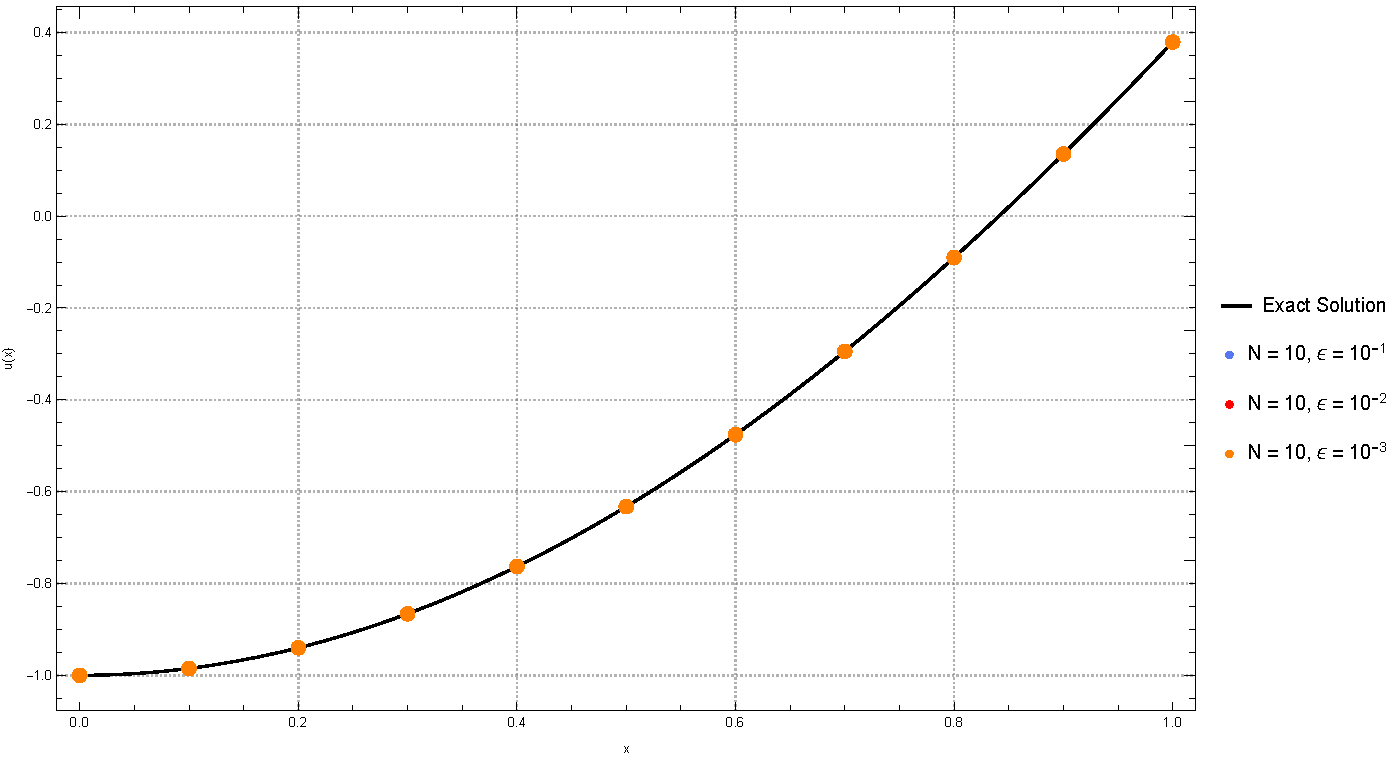
\includegraphics[width=0.6\linewidth]{N_10.pdf}} a) \\
\end{minipage}
\vfill
\begin{minipage}[h]{1\linewidth}
\center{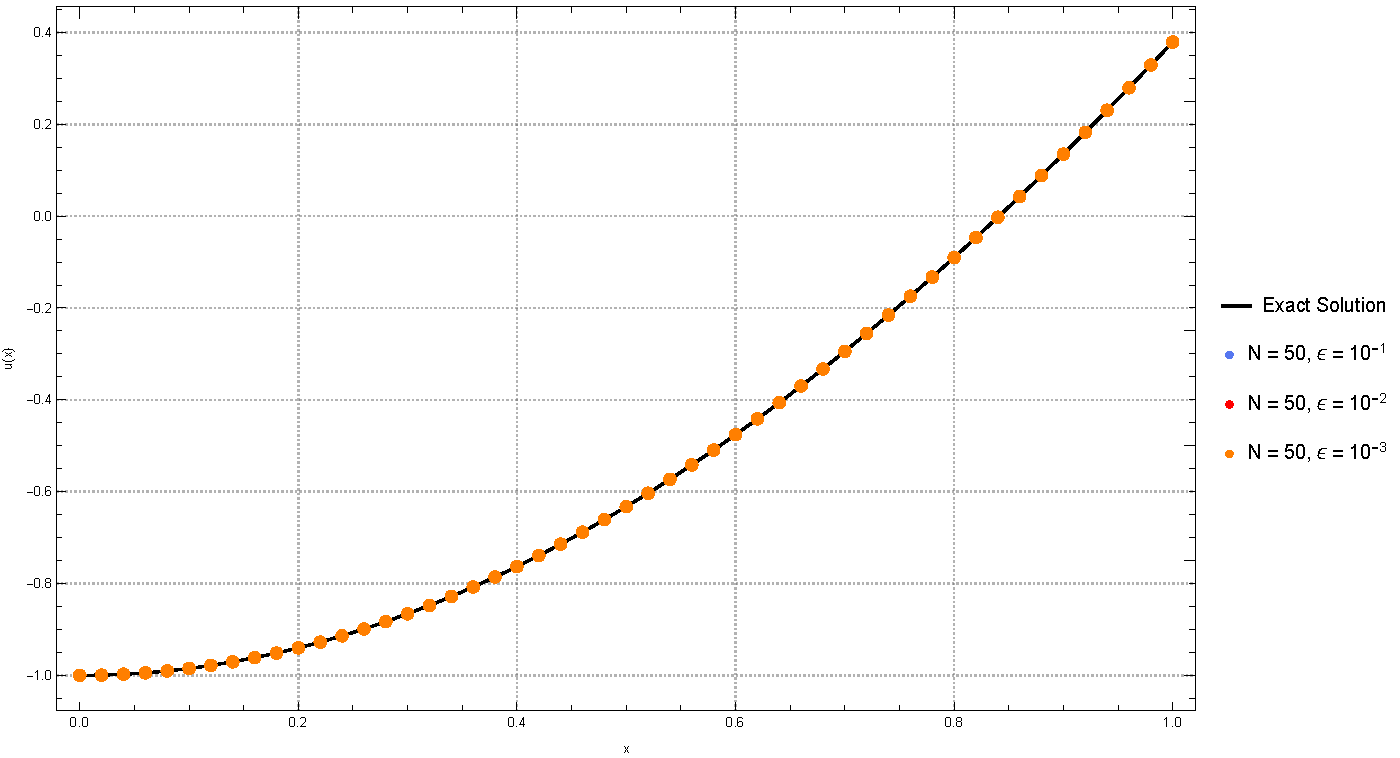
\includegraphics[width=0.6\linewidth]{N_50.pdf}} b) \\
\end{minipage}
\vfill
\begin{minipage}[h]{1\linewidth}
\center{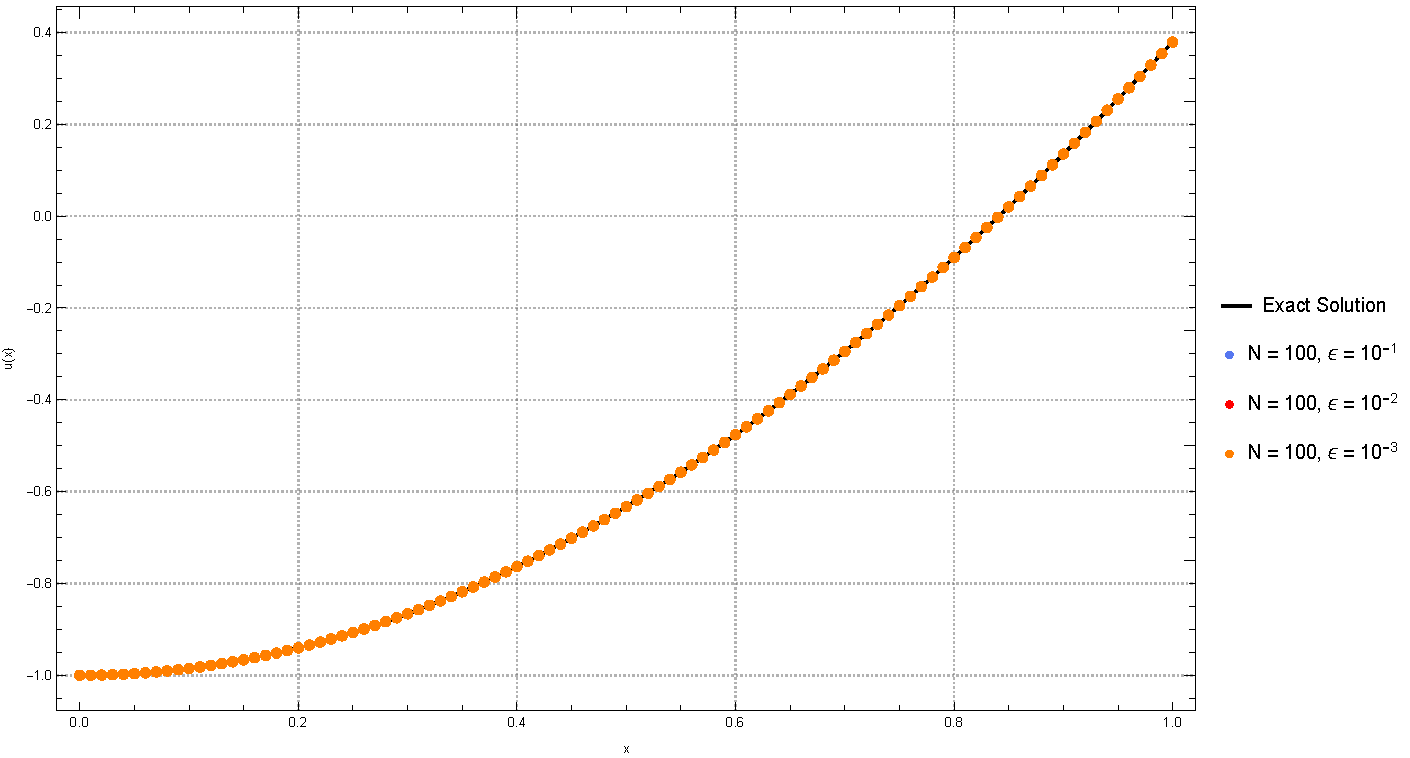
\includegraphics[width=0.6\linewidth]{N_100.pdf}} c) \\
\end{minipage}
\vfill
\caption{Решение задачи Коши для ОДУ $u' = (2-u)\tan(x)$, $u(0) = -1$, $x\in [0,1]$ методом предиктор-корректор при a) $N = 10$, b) $N = 50$, c) $N = 100$ для $\varepsilon = 10^{-1},\;10^{-2},\;10^{-3}$}
\label{ris:1}
\end{figure}

\newpage
\subsection{Задание Б}
\textbf{Значения $B_{ki}$ для $k,i = \overline{0,7}$}\\
$B_{0, 0} =  1 $\\
$B_{1, 0} = \frac{3}{2}, B_{1, 1} =  -\frac{1}{2} $\\
$B_{2, 0} = \frac{23}{12} ,B_{2, 1} =  -\frac{4}{3}                 ,B_{2, 2} =  \frac{5}{12} $\\
$B_{3, 0} =  \frac{55}{24} ,B_{3, 1} = -\frac{59}{24}                 ,B_{3, 2} =  \frac{37}{24}                   ,B_{3, 3} =  -\frac{3}{8}$\\
$B_{4, 0} =  \frac{1901}{720} ,B_{4, 1} =  -\frac{1387}{360}                ,B_{4, 2} =  \frac{109}{30}                  ,B_{4, 3} =  -\frac{637}{360}                 ,B_{4, 4} =  \frac{251}{720}    $\\
$B_{5, 0} =  \frac{4277}{1440} ,B_{5, 1} =  -\frac{2641}{480}                 ,B_{5, 2} =  \frac{4991}{720}                  ,B_{5, 3} =  -\frac{3649}{720}                 ,B_{5, 4} =  \frac{959}{480}                  ,B_{5, 5} =  -\frac{95}{288}   $\\
$B_{6, 0} =  \frac{198721}{60480} ,B_{6, 1} =  -\frac{18637}{2520}                 ,B_{6, 2} =  \frac{235183}{20160}                  ,B_{6, 3} =  -\frac{10754}{945}                 ,B_{6, 4} =  \frac{135713}{20160}                  ,B_{6, 5} =  -\frac{5603}{2520}                 ,B_{6, 6} =  \frac{19087}{60480}      $\\
$B_{7, 0} =  \frac{16083}{4480}  ,B_{7, 1} =  -\frac{1152169}{120960}                 ,B_{7, 2} =  \frac{242653}{13440}                   ,B_{7, 3} =  -\frac{296053}{13440}                ,B_{7, 4} = \frac{2102243}{120960} ,B_{7, 5} = -\frac{115747}{13440}                  ,\\
B_{7, 6} =  \frac{32653}{13440}                 ,B_{7, 7} = -\frac{5257}{17280}   $\\


\textbf{Значения $b_{ki}$ для $k,i = \overline{0,7}$}\\
$b_{0, 0} = 1$\\
$b_{1, 0} = \frac{1}{2}      ,b_{1, 1} =  \frac{1}{2}    $\\
$b_{2, 0} = \frac{5}{12} ,b_{2, 1} =  \frac{2}{3}                 ,b_{2, 2} =  -\frac{1}{12}       $\\
$b_{3, 0} = \frac{3}{8} ,b_{3, 1} =  \frac{19}{24}                 ,b_{3, 2} =  -\frac{5}{24}                ,b_{3, 3} =  \frac{1}{24}    $\\
$b_{4, 0} = \frac{251}{720} ,b_{4, 1} =  \frac{323}{360}                 ,b_{4, 2} =  -\frac{11}{30}                ,b_{4, 3} =  \frac{53}{360}                 ,b_{4, 4} = -\frac{19}{720}            $\\
$b_{5, 0} = \frac{95}{288} ,b_{5, 1} =  \frac{1427}{1440}                 ,b_{5, 2} =  -\frac{133}{240}               ,b_{5, 3} =  \frac{241}{720}                ,b_{5, 4} =  -\frac{173}{1440}               ,b_{5, 5} =  \frac{3}{160}              $\\
$b_{6, 0} = \frac{19087}{60480}  ,b_{6, 1} =  \frac{2713}{2520}                  ,b_{6, 2} =  -\frac{15487}{20160}                ,b_{6, 3} =  \frac{586}{945}                 ,b_{6, 4} =  -\frac{6737}{20160}                ,b_{6, 5} =  \frac{263}{2520}                 ,b_{6, 6} =  -\frac{863}{60480}             $\\
$b_{7, 0} = \frac{5257}{17280} ,b_{7, 1} =  \frac{139849}{120960}                  ,b_{7, 2} =  -\frac{4511}{4480}                 ,b_{7, 3} =  \frac{123133}{120960}                 ,b_{7, 4} =  -\frac{88547}{120960}                ,b_{7, 5} =  \frac{1537}{4480}                 ,b_{7, 6} =  -\frac{11351}{120960}              ,\\
b_{7, 7} =  \frac{275}{24192}$\\

\textbf{Значения $\gamma_{i}$ (Explicit formula) и $\overline{\gamma_{i}}$ (Implicit formula) для $i = \overline{0,7}$}\\
$\gamma_0 = 1, \gamma_1  = \frac{1}{2}, \gamma_2  =  \frac{5}{12}, \gamma_3  =  \frac{3}{8} , \gamma_4  =  \frac{251}{720}, \gamma_5  = \frac{95}{288}, \gamma_6  = \frac{19087}{60480}, \gamma_7  =  \frac{5257}{17280} $\\
$\overline{\gamma_0} = 1, \overline{\gamma_1} =  -\frac{1}{2}, \overline{\gamma_2} =  -\frac{1}{12}, \overline{\gamma_3} = -\frac{1}{24}, \overline{\gamma_4} = -\frac{19}{720}, \overline{\gamma_5} = -\frac{3}{160}, \overline{\gamma_6} = -\frac{863}{60480}, \overline{\gamma_7} = -\frac{275}{24192}$


\newpage
\section{Вывод}
Методом предиктор-корректор решена задача Коши для ОДУ $u' = (2-u)\tan(x)$, $u(0) = -1$, $x\in [0,1]$. Вычислены коэффициенты $B_{ki}$, $b_{ki}, \gamma_i$, $\overline{\gamma}_i$, $k,i = \overline{0,7}$ членов ряда разностного уравнения для экстраполяционной и интеполяционной формул Адамса в случае использования интерполяционных многочленов Лагранжа и Ньютона.

Метод предиктор-корректор показал значительно большую точность, чем ранее рассмотренные методы решения дифференциальных уравнений.
\end{document} 